\graphicspath{{chapters/chapter5/}}
\chapter{Results} \label{chapter5}
\label{exp_Results}
\section{Experiments}
% Please add the following required packages to your document preamble:
% \usepackage{multirow}
\begin{table}[]
\begin{tabular}{|l|l|l|l|l|}
\hline
 &
  Name &
  Base &
  \begin{tabular}[c]{@{}l@{}}Classification \\ Head(s)\end{tabular} &
  Loss Function \\ \hline
\multirow{4}{*}{\begin{tabular}[c]{@{}l@{}}Single Task \\ Learning (STL) \\ for diagnosis \\ prediction\end{tabular}} &
  \textit{IncNet} &
  IncNet &
  F.C. &
  Cross-Entropy \\
 & \textit{IncNet*+L.R.}               & IncNet* & L.R.     & L2 penalty     \\
 & \textit{ResNet}                     & ResNet  & F.C.     & Cross-Entropy \\
 & \textit{ResNet*+L.R.}               & ResNet* & L.R.     & L2 penalty     \\ \hline
\multirow{3}{*}{\begin{tabular}[c]{@{}l@{}}Muli Task Learning\\ (MTL) for Concepts \\ prediction\end{tabular}} &
  \textit{IncNet$_{MTL}$} &
  IncNet &
  F.C. x 7 &
  Cross-Entropy \\
 & \textit{IncNet*$_{MTL}$+L.R.}       & IncNet* & L.R. x 7 & L2 penalty     \\
 & \textit{ResNet*$_{MTL}$+L.R.}       & ResNet* & L.R. x 7 & L2 penalty     \\ \hline
\multirow{6}{*}{\begin{tabular}[c]{@{}l@{}}Concept Bottleneck \\ Models (CBM) \\ for diagnosis \\ prediction\end{tabular}} &
  \textit{Ind | IncNet$_{MTL}$} &
  IncNet &
  L.R. &
  L2 penalty \\
 & \textit{Seq | IncNet$_{MTL}$}       & IncNet  & L.R.     & L2 penalty    \\
 & \textit{Ind | IncNet*$_{MTL}$+L.R.} & IncNet* & L.R.     & L2 penalty     \\
 & \textit{Seq | IncNet*$_{MTL}$+L.R.} & IncNet* & L.R.     & L2 penalty     \\
 & \textit{Ind | ResNet*$_{MTL}$+L.R.} & ResNet* & L.R.     & L2 penalty    \\
 & \textit{Seq | ResNet*$_{MTL}$+L.R.} & ResNet* & L.R.     & L2 penalty     \\ \hline
\end{tabular}
\caption*{*weights are frozen}
\caption{Representation of models used for experiments. F.C.: Fully Connected layer; L.R.: Logistic Regression.}
\label{table:modelsTable}
\end{table}
The goal of this work, is to develop a model able to detect Melanoma in dermoscopic images of skin lesions, by learning first a set of human-understandable concepts. \\
To do this, the Concept Bottleneck Framework (Sec. \ref{sectionCBM}) was employed, by designing models that first predict the clinical attributes from 7-poin checklist method(Sec. \ref{7ptRule}) and then use those for the final diagnosis of the lesion. \\
These models have then been compared with the more standard Single Task Learning approaches, which learn the diagnosis end-to-end without intermediate concepts.\\ 
All proposed models, shown in Table~\ref{table:modelsTable}, use an IncNet or a ResNet pretrained over ImageNet as base model. The class-specific layer of either models was replaced with a trainable layer related to the task. \\

\subsection{Single Task Learning for Diagnosis prediction}
Single Task Learning architectures are end-to-end models $g$ that from an input $x$ (Dermatoscopy image) predict directly the diagnosis, by extracting hidden features $h=f(x)$, and by using them to predict $\hat{y}_{DIAG}=g(f(x))$, by means of a classification head. Figure~\ref{fig:StLimage} shows a standard representation for a STL model.\\
The first two implementation are the \emph{IncNet} and the \emph{ResNet}, which use respectively as base $f$ an InceptionV3 and a ResNet101V2 imported from TensorFlow library \cite{tensorflow2015-whitepaper}.
In both networks, the final layer was replaced with a Fully Connected layer, the classification head $g$, specific to the Diagnosis task and categorical cross-entropy loss was used. Training has been done using a custom Keras Sequence with augmentation on training set, by flipping and cropping images, on 250 epochs with a patience of 50 epochs and a learning rate of
0.001 for ADAM optimizer(See Sec. \ref{IncNet}, \ref{ResNet} for more training details).\\
The experiments \emph{IncNet*+L.R.} and \emph{ResNet*+L.R.} were developed similarly to the method presented in the work of Kawahara et al.\cite{Kawahara}. By using respectively an InceptionV3 and a ResNet101V2 as base $f$ of the networks. The models were initialized with weights trained on the ImageNet dataset; keeping them frozen, they were employed to extract a set of features $h=f(x)$. Extracted features $h$ and related DIAG labels, were employed then, for the training of the Logistic Regression model $g$ added to the head of the network. The Logistic Regression models were implemented by using the scikit learn library \cite{scikit-learn}, in which a L2 penalty loss function is used. Logistic Regression model was trained using the extracted features.
\subsection{Multi Task Learning for Concepts prediction} \label{sectionMTL}
Multi task learning models have the form of $\{g_t(f(x)),\; \forall t \in \{ PN, BWV, \hdots \} \}$ where $f$ performs the extraction of hidden features from a base model and $g_t$ predicts the 7 tasks of the 7-point checklist rule, according to Table~\ref{table:3}. General architecture of MTL models is showed in Figure~\ref{fig:x_cimage}.\\ 
The first MTL model presented is the \emph{IncNet$_{MTL}$}, in which an InceptionV3 was joined to a block of Dense layer, followed by 7 Fully Connected layers, each of them related to one of the 7 tasks. For each block, Categorical Cross-Entropy loss function was implemented. The resulting model was trained on the training set over 200 epochs with a patience of 30, and a stochastic gradient descent (SGD) having a learning rate of 0.001 as optimization algorithm(See Sec. \ref{MtlIncNet} for more training details).\\
\emph{IncNet*$_{MTL}$+L.R.} and \emph{ResNet*$_{MTL}$+L.R.} models, use a frozen base model trained on ImageNet to extract features that are then used ad input to 7 different Logistic Regressions (one per task). Each  Logistic Regression model was trained using extracted features as input and each task's label as ground truth.
\subsection{Concept-Bottleneck Models for Diagnosis prediction}
Concept Bottleneck architectures have the form $\tilde{g}_{DIAG} \left( g_{PN} \left( f(x) \right),\;  g_{BWV} \left( f(x) \right),\; \hdots \right)$, where $f(x)$ performs the features extraction from a base model, $g_t$ the intermediate concept prediction for every attribute $t$ in the 7-point checklist (Sec. \ref{7ptSection}) and $\tilde{g}$ performs the prediction of the main classification task using the predicted concepts $\hat{c} = \{g_t(f(x)),\; \forall t \in \{ PN, BWV, \hdots \} \}$ represented in Table~\ref{table:3}, related to the 7pt checklist rule. Independent and sequential architecture were implemented by joining the models for concepts predictions to a Logistic Regression classifier. \\
In the Independent models the functions to predict the concepts are trained Independently from the one to predict the main task. Three different approaches to predict the tasks have been described in the previous section(Sec. \ref{sectionMTL}). The function to predict the diagnosis is trained using the ground truth for the concepts as input.
Conversely, in the Sequential model the two models are trained one after the other. First the concepts predictor is trained to generate the prediction $\hat{c}$. Then the logistic regression to predict the diagnosis is trained on the predicted concepts $\hat{c}$.\\
General architecture of CBM is showed in Figure \ref{fig:CBMimage}, where as $g(f(x))$ it takes one of the proposed models for concepts prediction, and as $\tilde{g}(\cdot)$ a Logistic Regression model.
\begin{figure}[]
\centering
  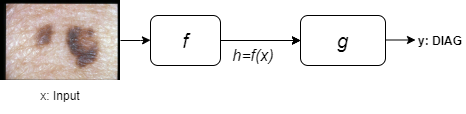
\includegraphics[width=.7\linewidth]{images/model/STL.png}
  \caption{Architecture for end-to-end models that go directly from raw input $x$ to final target $y$.}
  \label{fig:StLimage}
\end{figure}


\begin{figure}[]
\centering
  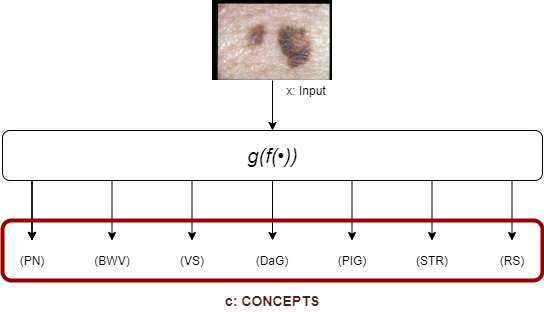
\includegraphics[width=.7\linewidth]{images/model/MTL (2).png}
  \caption{Architecture for MTL models}
  \label{fig:x_cimage}
\end{figure}

\begin{figure}[]
\centering
  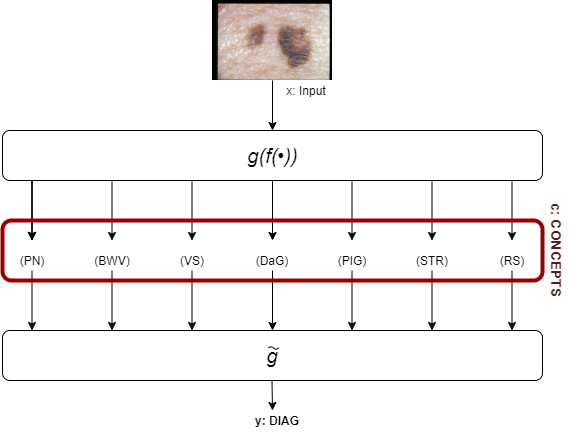
\includegraphics[width=.7\linewidth]{images/model/CBm (1).png}
  \caption{General architecture for Concept Bottleneck models}
  \label{fig:CBMimage}
\end{figure}
\subsection{7-point Checklist Rule}
7-point Checklist Rule is applied using the ground truth concepts from the test set, and it diagnoses Melanoma if a score greater than or equal to 3 was obtained.

\section{Results}
The performance of all proposed methods for lesion identification and melanoma diagnosis was evaluated using accuracy, recall, F1 score on MEL label and precision, which can be defined as follows:
\begin{equation}
    Accuracy = \frac{tp + tn}{tp + tn + fp +fn}
\end{equation}
\begin{equation}
    Recall = \frac{tp}{tp +fn}
\end{equation}
\begin{equation}
    Precision = \frac{tp}{tp + fp}
\end{equation}
\begin{equation}
    F1 score =2 \cdot \frac{precision \cdot recall}{precision + recall}
\end{equation}
where $tp$,$tn$,$fp$ and $fn$ refer to true positive, true negative, false positive, and false negative, respectively. The baseline results obtained from proposed system for melanoma diagnosis are presented in Table~\ref{table:results}, and accuracy on concepts predictions, is shown in Table~\ref{table:ConceptsAccuracy}.
The performance of the models were measured by performing stratified 5-fold cross-validation on the test set. The test set was divided into 5 folds, balanced according to the true label of diagnosis.\\ \\
In Single task learning prediction, the best performance was achieved by \emph{ResNet} model trained using Transfer Learning, which obtained about $81.25\pm3.28\%$ in Accuracy metric. Comparable performance were obtained by \emph{ResNet*+L.R.}, even if it wasn't trained on Derm7pt images; this model shows better performance even than \emph{IncNet}. Hierarchies implementing ResNet101v2 showed the best metrics in single task learning, and fine-tuned models remained the most performing. However satisfactory results were also obtained by simply freezing the weights in \emph{IncNet*} and \emph{ResNet*} where, the feature extractors were learned for general images in ImageNet. \\\\
Also for the MTL models we find that the fine-tuned models performed better than models in which the weights were frozen. Table~\ref{table:ConceptsAccuracy} summarizes the performance of models in predicting the concepts alone. \emph{IncNet$_{MTL}$} trained on Derm7pt, reports the best accuracy in concepts predictions, with an average value of $66.97 \pm5.84\%$, compared to $65.93\pm5.03\%$ and $65.93\pm4.84  \%$ obtained with \emph{IncNet*$_{MTL}$+L.R.} and \emph{ResNet*$_{MTL}$+L.R.} models.\\\\
The best bottleneck model were the \textit{Seq | IncNet$_{MTL}$} and \textit{Seq | ResNet$_{MTL}$} that achieved $77.50\pm8.07\%$ and $76.56\pm3.13\%$ accuracy respectively on Diagnosis prediction.\\
In each CBM implementations, Sequential bottleneck models, seem to be more accurate than Independent models, also if the sequential $f$ model is trained on predicted concepts, while independent $f$ model is trained on the true concepts.
\\\\
The model that accomplish the best performance was the one with the "black-box" nature, the \emph{ResNet} model. STL learning therefore remains the finest, but it can't provide an explanation of how it predicts the final target $y$, unlike CBM that provides a set of human-understandable specified concepts for a clear explanation.
\\\\
The clinical rule used by dermatologists still seems to be the most effective. In fact, by applying the ground truth score of each concepts taken from the test set, it obtains the best accuracy compared to the proposed architectures. In particular, it showed the best results for the F1 score metric related to the MEL label, obtaining $ 78.43\pm4.77 \% $ far higher than the scores achieved by the proposed models.\\
For more details on model predictions see section \ref{chapter7}, which shows the related confusion matrices for each architecture.
\\\\
Overall, the architectures developed perform adequately and they stand up to other works proposed in the literature.
Comparing with other approaches that used the same dataset is challenging as often different subsets of the data are used and especially, because this work only considers melanoma and nevus cases of the Derm7pt dataset.
In \cite{Kawahara,mtl7ptCoppola} the DIAG task and the 7 tasks were put on the same level without taking into consideration any possible intermediate implementation;
Kawahara et al.~\cite{Kawahara} achieved an accuracy\footnote{Kawahara et al.\cite{Kawahara} results refer to experiment \textit{x-combine}, which uses additional data during training} of $74.2\%$ but taking into consideration all the labels of the DIAG task (BCC, NEV, MEL, MISC, SK) and not only MEL and NEV labels; while they achieved an average value of $73.6\%$ on concepts prediction.
Coppola et al.~\cite{mtl7ptCoppola} achieved an accuracy\footnote{Coppola et al.\cite{mtl7ptCoppola} results refer to experiment \textit{binary}, which considers only 2 output classes for DIAG task} of $77.2\%$ and an average value of $61.3\%$ on the 7 attributes prediction.\\
The \textit{Seq | IncNet$_{MTL}$} implementation performed better than the 2 results achieved in \cite{Kawahara,mtl7ptCoppola}, providing a better explanation of how the diagnosis was computed, although it must be remembered that it only distinguishes between NEV and MEL labels.


\begin{table}[]
\begin{tabular}{|l|c|c|c|c|}
\hline
\textbf{Model}  & \multicolumn{1}{c|}{Accuracy}      & \multicolumn{1}{c|}{Recall}  & \multicolumn{1}{c|}{F1 Score} & \multicolumn{1}{c|}{Precision}\\ \hline
\emph{IncNet}   & $78.43 \pm 2.50$    & $74.36\pm12.17$     &  $64.82\pm4.75$   & $75.13 \pm 9.02$\\
\emph{ResNet}    & \boldsymbol{$81.25 \pm 3.28$}   & $76.69\pm 14.68$ &    \boldsymbol{$67.96 \pm 7.15$}& \boldsymbol{$78.68 \pm 6.98$}\\
\emph{IncNet*+L.R.}   & $74.06\pm6.60$    & $71.17\pm10.96$ & $60.75\pm9.74$& $70.37\pm 6.98$             \\ 
\emph{ResNet*+L.R.}   & $80.31\pm2.89$      & \boldsymbol{$76.77\pm 12.80$} & $67.79\pm7.02$ & $77.37\pm14.29$          \\ 

\hline
\textit{Ind | IncNet$_{MTL}$} & $77.50 \pm8.36$ & $74.45\pm13.62$ & $65.12\pm12.50$ & $74.42\pm14.27$\\ 
\textit{Seq | IncNet$_{MTL}$} & \boldsymbol{$77.50 \pm 8.07$}& \boldsymbol{$74.72 \pm 12.61$} & \boldsymbol{$65.60 \pm 11.33$}&\boldsymbol{$74.60 \pm 13.96$}\\ 


\textit{Ind | IncNet*$_{MTL}$+L.R.} & $69.06\pm6.80 $& $68.56 \pm 8.25$  & $57.96\pm 8.70$&$66.64\pm 17.08$  \\ 
\textit{Ind | ResNet*$_{MTL}$+L.R.}  & $74.69\pm3.88$     & $72.96 \pm 6.04$  & $63.19 \pm 3.75$& $71.51 \pm 13.21$       \\ 
 
\textit{Seq | IncNet*$_{MTL}$+L.R.} & $71.88\pm7.33$      & $70.36\pm9.32$   & $59.97 \pm 9.93$&$ 68.76\pm 16.05$         \\ 
\textit{Seq | ResNet*$_{MTL}$+L.R.}  & $76.56\pm 3.13$ & $74.07\pm7.41 $& $64.56 \pm 3.64$& $ 73.18 \pm 11.68$  \\\hline
 \textit{7pt-Checklist Algorithm} & \boldsymbol{$83.44\pm4.38$} &  \boldsymbol{$86.28\pm8.96$} &\boldsymbol{$78.43\pm4.77$} & \boldsymbol{$82.03\pm15.31$} \\ \hline
\end{tabular}
\caption*{*weights are frozen}
\caption{Accuracy, recall, F1 score on MEL label and precision on DIAG task, calculate by splitting the test set in 5 subsets. }
\label{table:results}
\end{table}

\begin{landscape}
\begin{table}


\begin{tabular}{|l|c|c|c|c|c|c|c|c|}
 \hline
 \textbf{Model} & \textbf{PN} & \textbf{DaG}& \textbf{BWV}& \textbf{PIG}& \textbf{STR}& \textbf{RS}& \textbf{VS} & \textbf{avg}\\
 \hline

\textit{IncNet*$_{MTL}$+L.R.} & \boldsymbol{$58.13\pm8.58$} & $57.50\pm4.01$ & $79.06\pm7.07$ & $57.81\pm4.64$ & $65.94\pm3.03$ & $70.31\pm2.80$ & $72.81\pm5.10$ & $65.93\pm5.03$\\
\textit{ResNet*$_{MTL}$+L.R.} & $57.81\pm5.59$ & $55.94\pm2.50$ & \boldsymbol{$80.31\pm6.30$} &\boldsymbol{$58.44\pm6.22$} &$66.25\pm4.49$ & $70.31\pm4.08$ & $72.50\pm4.70$ & $65.93\pm4.84$ \\
\textit{IncNet$_{MTL}$} & $52.19\pm7.24$ & \boldsymbol{$57.51\pm4.12$} & $75.94\pm7.30$ & $58.13\pm4.57$ & \boldsymbol{$71.25\pm6.60$} &\boldsymbol{$72.19\pm5.36$
 } & \boldsymbol{$81.56\pm5.71$} & \boldsymbol{$66.97\pm5.84$}\\
\hline
\end{tabular}
\caption*{*weights are frozen}
\caption{Mean Accuracy and standard deviation on concepts prediction computed with Stratified K-Fold.}
\label{table:ConceptsAccuracy}

\end{table}
\end{landscape}

